\section{Evaluating causal models}

Consider the joint probability measure $P:\mathcal{H}\times \mathcal{A}\times \mathcal{I}\times \mathcal{Q}\times \mathcal{V}\to [0,1]$ defined by the following composition of $P_H$ and kernels in the model $\mathscr{M} = \langle P_H, \theta, \pi, \phi, \mu \rangle$:

\begin{center}
\begin{tikzpicture}[-latex ,auto ,node distance =1 cm and 4cm ,on grid ,
semithick ,
variable/.style ={ circle ,top color =white , 
draw , text=blue , minimum width =1 cm},
kernel/.style={rectangle,draw}
]
\node[kernel] (Kmu) [right] {$\mu$};
\node[kernel] (Kphi) [above left = 2cm and 2cm of Kmu] {$\phi$}
    edge[bend left] (Kmu);
\node[kernel] (Ktheta) [above left = 1cm and 2cm of Kphi] {$\theta$}
    edge[bend left] (Kphi);
\node[kernel] (Kpi) [below left = 1cm and 2cm of Kphi] {$\pi$}
    edge[bend right] (Kphi);
\node[inner sep=0pt] (S) [below left = 1cm and 2cm of Ktheta] {}
    edge[bend left] (Ktheta)
    edge[bend right] (Kpi)
    edge[bend right = 50] (Kmu);
\node (A) [left = 1cm of S] {$P_H$}
    edge[-] (S);
\draw (Kmu.east) -- +(1,0);
\end{tikzpicture}
\end{center}

Define the related distribution $P_q$ generated by $\mathscr{M}_q = \langle P_H, \delta_{qq'}, \theta, \pi, \phi, \mu\rangle$ composed as in the image below. $P_q$ is analogous to $P(\cdot | do(q))$ in the Causal Bayesian Network framework.

\begin{center}
\begin{tikzpicture}[-latex ,auto ,node distance =1 cm and 4cm ,on grid ,
semithick ,
variable/.style ={ circle ,top color =white , 
draw , text=blue , minimum width =1 cm},
kernel/.style={rectangle,draw}
]
\node[kernel] (Kmu) [right] {$\mu$};
\node[kernel] (Kphi) [above left = 2cm and 2cm of Kmu] {$\phi$}
    edge[bend left] (Kmu);
\node[kernel] (Ktheta) [above left = 1cm and 2cm of Kphi] {$\theta$}
    edge[bend left] (Kphi);
\node[kernel] (Kpi) [below left = 1cm and 2cm of Kphi] {$\pi$};
\node[inner sep=0pt] (S) [below left = 1cm and 2cm of Ktheta] {}
    edge[bend left] (Ktheta)
    edge[bend right] (Kpi)
    edge[bend right = 50] (Kmu);
\node (A) [left = 1cm of S] {$P_H$}
    edge[-] (S);
\node (B) [left = 1.5cm of Kphi] {$\delta_{qq'}$}
    edge (Kphi);
\draw (Kmu.east) -- +(1,0);
\end{tikzpicture}
\end{center}

\begin{definition}[Policy estimator]
A policy estimator $\mathscr{E}:(A\times I \times V)^n\to (Q\to \Delta(I\times V))$ maps a dataset of triples $D=\{(a_i,i_i,v_i)|i\leq n\}$ to an estimate $Q\to \Delta(i,v)$:
\begin{align}
    \mathscr{E}(D) = f(q;i,v)
\end{align}
\end{definition}

\begin{definition}[$\mathscr{E},D$-counterfactual identifiability]
A causal model $\langle P_H, \mu,\pi,\phi,\theta\rangle$ with is $\mathscr{E},D$-counterfactually identifiable if 

\begin{align}
    \mathscr{E}(D)=P_q(i,v)
\end{align}
\end{definition}


\begin{definition}[$\mathscr{E},D$-conditional Identifiability]
A causal model $\langle P_H, \mu,\pi,\phi,\theta\rangle$ is $\mathscr{E},D$-conditionally-identifiable if 

\begin{align}
    \mathscr{E}(D)=P(i,v|q)
\end{align}
\end{definition}

Figure \ref{fig:venn_diagram} illustrates the relationship between different notions of identifiability. Counterfactual and conditional identifiability differ on the choice of \emph{evaluation scheme}.

\begin{figure}
    \centering
    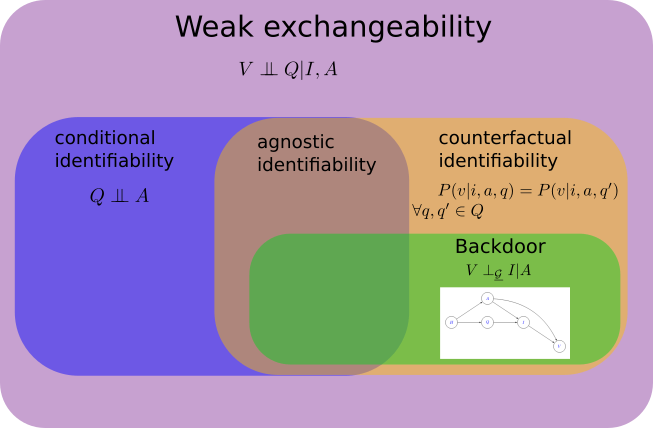
\includegraphics{venn_diagram.png}
    \caption{Relationship between conditional and counterfactual identifiability}
    \label{fig:venn_diagram}
\end{figure}

\subsection{Evaluation schemes}

Given a causal model $\mathscr{M}=\langle P_H, \pi, \theta, \phi, \mu\rangle$ and a cost function $C:\Delta(I\times V)\to \mathbb{R}$, we typically want to find $q$ minimising $C(K(q;(i,v)))$ for some evaluation kernel $K:Q\to \Delta(I\times V)$. We would expect the kernel $K$ to come from some evaluation scheme $\mathscr{S}:\{\mathscr{M}\}\times Q\to \Delta(I\times V)$. There are at least two plausible candidates for what this scheme should be:
\begin{enumerate}
    \item $\mathscr{S}_{ca}(\mathscr{M}) = P_q(i,v)$
    \item $\mathscr{S}_{con}(\mathscr{M})=P(i,v|q)$
\end{enumerate}

Counterfactual and conditional identifiability correspond to the use of $\mathscr{S}_{ca}$ and $\mathscr{S}_{con}$ respectively. Also, in a loose sense, $\mathscr{S}_{ca}$ accords with ``causal decision theory'' and  $\mathscr{S}_{con}$ accords with ``evidential decision theory''.

Two examples illustrate that we want to avoid naively adopting either scheme.

\subsubsection{Example: useless medicine}

Useless medicine is an example in which $\mathcal{S}_{con}$ gives an intuitively incorrect result while $\mathcal{S}_{ca}$ gives an intuitively correct one.

$S\in \{0,1\}$ is information on whether or not someone is sick, $I=\{0,1\}$ is a variable representing whether or not they received treatment and $V=\{0,1\}$ is a variable representing whether or not they recovered. A dataset of pairs $(i,v)$ is collected to determine the medicine's efficacy, and a prescription policy $\hat{q}$ is created based on the estimated costs $C(\tilde{P}(i,v|do(q)))$.  The experimenter is aiming to maximise the probability of recovery, while avoiding unnecessary treatment: $C(P(i,v))=-\mathbb{E}[V-0.5I]$. 

There are no observed covariates, $A=\emptyset$, and $Q=\{0,1\}$ are the ``don't treat'' and ``always treat'' policies respectively. $H$ is simply the sickness status of the patient $H=S$.

The kernels and $P_H$:
\begin{itemize}
    \item $P_H(s=1) = 0.5$
    \item $\mu(i,s,v) =\delta_{sv}$; Sick people always recover, healthy people don't
    \item $\pi(s,q)=\delta_{sq}$; Only sick people were treated
    \item $\phi(q,i)=\delta_{qi}$; if $Q=1$ treat, otherwise don't
\end{itemize}

We have two choices of prescription policy - $\hat{q}=0$ and $\hat{q}=1$. Using $\mathscr{S}_{ca}$:

\begin{align}
    P_q(i,v) &= \sum_{s} \mu(i,s,v) \pi_{q}(s,q') \phi(q',i) P_H(s) \\
                         &= \sum_{s} \delta_{sv} \delta_{q'q} \delta_{q'i} P_H(s) \\
                         &= \delta_{qi} \sum_{s} \delta_{sv} P_H(s) \\
                         &= 0.5 \delta_{qi} (\delta_{v1} + \delta_{v0})
\end{align}

Minimising the cost function here would recommend not treating, which appears to be the correct decision in this case.

on the other hand, using $\mathscr{S}_{con}$:

\begin{align}
    P(i,v|q) = \delta_{qv}
\end{align}

Minimising the cost function here would recommend always treating, which seems incorrect.

Note that (not shown here) useless medicine is conditionally identifiable but not counterfactually identifiable.

\subsubsection{Example: state space optimal control}

Consider the case of a discrete linear time-invariant control system with state given by
\begin{align}
    \mathbf{x}_{k+1} &= A\mathbf{x}_k + B\mathbf{i}_k\\
    \mathbf{x}_0 &= x(0)
\end{align}

Where 
\begin{itemize}
    \item $\mathbf{x}_\cdot \in \mathbb{R}^n$
    \item $\mathbf{i}_\cdot \in \mathbb{R}^m$
    \item $A\in \mathbb{R}^{2n}$
    \item $B\in \mathbb{R}^{2m}$
    \item $x(0)\in \mathbb{R}^n$ is some constant
\end{itemize}

We assume the system is Markovian - that is, $\mathbf{x}_{k+1}$ depends on nothing besides $\mathbf{x}_k$ and $\mathbf{i}_k$. 

In the causal model framework given here, $a=\mathbf{x}_k$ and $v=\mathbf{x}_{k+1}$ while $i=\mathbf{i}_k$. The control policy $Q\in \mathbb{R}^{nm}$ is a matrix such that $\mathbf{i}_k = Q\mathbf{x}_k$. The history $h=(a,q)$.

The assumption of Markovianity gives strong policy exchangeability. We have weak exchangeability directly from this assumption: $v_{k+1}$ does not depend on anything conditioned on $\mathbf{x}_k$ and $\mathbf{i}_k$. We note that this remains true if $\mathbf{i}_k = Q\mathbf{x}_k + \epsilon$ for some noise $\epsilon \in \mathbb{R}^m$, which gives strong exchangeability.

Covariate stability does not hold in general; given some a control policy $Q$, we regard this choice as fixed for all values of $k$. Thus in general $\mathbf{x}_k$ depends on $Q$ for all $k\neq 0$.

In summary, the control system as defined here is counterfactually identifiable but not conditionally identifiable.

It is straightforward to show that, given a cost $C(P(i,v))$, choosing $q$ such that $C(P_q(i,v))$ is minimised corresponds to the greedy policy $q$. I don't yet know whether choosing $q$ such that it minimises $C(P(i,v|q))$ corresponds to an optimal policy in the undiscounted case, but it seems plausible.

The following argument chiefly serves to illustrate that parametrising the model such that covariate stability holds can make analysis easier.

We have $v$ as before, $a=\mathbf{x}_0$, $i=[\mathbf{i}_k \mathbf{i}_{k-1} ... \mathbf{i}_0]^T$ and $Q\in \mathbb{R}^{n^2m}$ is such that $i = Q \mathbf{x}_0$.

The criterion of \emph{controllability} asks if it is possible to find a control sequence $i$ such that for any $\mathbf{x}_0$ we can arrive at a target value $\hat{\mathbf{x}}$. We will call the problem of $k$-controllability the question of whether this is possible within $k$ steps.

Note that we can write the $k$-step transition as
\begin{align}
    \mathbf{x}_k = A^k \mathbf{x}_0 + \sum_{j=0}^{k-1} A^j B \mathbf{i}_j
\end{align}

Alternatively, using $i=[\mathbf{i}_k \mathbf{i}_{k-1} ... \mathbf{i}_0]^T$ and defining $R=[B\;AB\; ...\;A^{k-1}B]$ we have

\begin{align}
    Ri &= \mathbf{x}_k - A^k \mathbf{x}_0 \\
       &\overset{def}{=} \mathbf{x}_T
\end{align}

This equation has a solution iff $RR^\dagger \mathbf{x}_T = \mathbf{x}_T$. This is true for all $\mathbf{x}_T$ iff $RR^\dagger = I$, which is true iff $\text{rank}(R)=n$.

Suppose $k=n$ and $\text{rank}(R) < n$. We know that the submatrices $B, AB, ...,A^{n-1}B$ must be linearly dependent. Then $A^{n-1}B = \sum_{j=0}^{n-2} u_j A^j B$. The matrix $A^n B$ can therefore be written $A^n B = \sum_{j=0}^{n-2} u_j A^{j+1} B= \sum_{j=0}^{n-3} u_j A^{j+1} B + u_{n-2} \sum_{j=0}^{n-2} u_j A^j B$, so adding $A^n B$ to the collection of submatrices doesn't increase the rank. Therefore a discrete linear time-invariant control system is controllable iff it is $n$-controllable.

\subsection{The Case for Agnostic Evaluation}

In both cases above, it could be argued that the problematic causal models are misspecified. In the useless medicine case, our intuition tacitly acknowledges that it must be possible to avoid prescribing medicine to someone who is sick, even if the model forbids it. In the case of the control system, it could be argued that the policy is ``really'' being chosen prior to $x_1$ being realised, so that $x_1,x_2,...$ should all be properly regarded as downstream of the policy (as in the reparametrisation). 

This section argues that there isn't an evaluation scheme that is satisfactory for every causal model, but for models where $\mathscr{S}_{ca} = \mathscr{S}_{con}$, either scheme is likely to be satisfactory.

The argument below is a work in progress at this stage.

Consider a causal model $\mathscr{M}$ of the problem of choosing a function $K:Q\to \Delta(V)$. That is, the interventions $I$ correspond to a set of functions $K_i:Q\to \Delta(V)$. We will also assume that $\phi$ depends only on $Q$ and that $Q=I$. That is, given a ``base'' evaluation kernel $K_q$, $\phi$ will yield a distribution over ``recommended'' evaluation kernels $\Delta(I)$. We will assume that $\phi$ takes a particular form: $\phi(q;i) = \delta_{\tilde{q}i}$ where $\tilde{q} \in \argmin_{q'} C(K_q(q'))\overset{def}{=} \argmin_{q'} C_q(q')$. Given some recommendation $\tilde{q}$, we have a mapping $\mu(\tilde{q},h;v)$ to outcomes.

Suppose there is an acceptable evaluation kernel $K_{q^*}$ for this problem. The following two criteria appear desirable:

\begin{itemize}
    \item \textbf{Self-recommendation}: $\phi(q^*;q^*)=1$
    \item \textbf{Model-optimality}: given the causal model $\mathscr{M}=\langle P_H, \pi,\theta,\phi,\mu\rangle$ (partly described above), $q^*\in \argmin_{q'} P(v|q')$
\end{itemize}

Self-recommendation asks that $K_{q^*}$ asserts its own correctness. Model-optimality asks that using $K_{q^*}$ to evaluate each $q$ yields a recommendation $\tilde{q}$ that is optimal under the distribution $P(v|q)$ generated by $\mathscr{M}$. This apparent endorsement of $K_{con}$ can be defended on the grounds that $P(v|q)$ by supposition represents the true relationship between $q$ and $v$.

\begin{theorem}[No universal evaluation kernel]
There exists a model $\mathcal{M}$ such that there is no kernel $K_{q^*}$ that satisfies both self-recommendation and model-optimality.
\end{theorem}

\begin{proof}
Consider a model $\mathscr{M}$ following the skeleton sketched above with $H=\{0,1\}$ and that generates the the distribution $P(h=1|q) = \delta_{q q_0}$. Suppose also that $C(P(v)) = -\mathbb{E}_P (V)$ and $\mu(q,h;v) = \delta_{hv}$. Finally, suppose that $K_{q_0}(q;v) = (1-\delta_{q q_0})\delta_{v1} + \delta_{v0} \delta_{q q_0}$. 

Then we have
\begin{align}
    P(v|q') &= \sum_h \mu (\phi(q'),h;v) P(h|q')\\
            &= \delta_{v q_0}\\
    \implies \argmin_{q'} C(P(v|q')) &= \{q_0\}
\end{align}

However, for $\hat{q}\neq q_0$,
\begin{align}
    \phi(q_0;q_0) &= \delta_{\tilde{q}q_0}\\
        \tilde{q} &= \argmin_{q'} C(K_{q_0}(q';v)) \\
    C(K_{q_0}(q_0;v)) &= 0\\
    C(K_{q_0}(\hat{q};v)) &= -1\\
    \implies q_0 &\not\in \argmin_{q'} C(K_{q_0}(q';v))\\
    \implies q_0 &\neq \tilde{q}
\end{align}
\end{proof}

This theorem shows that there are causal models for which any evaluation kernel must either endorse a different kernel, or sometimes recommend a policy $q$ that is not optimal by the true distribution.

The situation can be partly rescued however; below, we will show that $K_{ca}$ is always self-recommending and $K_{con}$ is trivially model-optimal. Thus, whenever these evaluation kernels agree, both have the properties of self-recommendation and model-optimality.

\begin{definition}[$\phi$-constant kernel]
    A kernel $K:Q\to \Delta(V)$ is $\phi$-constant if $\phi(q;i)=\phi(q';i)\implies K(q;v) = K(q';v)$ for all $q\in Q, i\in I, v\in V$.
\end{definition}

\begin{lemma}[$\phi$-constant functions are self-recommending]
A function $f_q$ is self-recommending if it is $\phi$-constant and $\phi$ breaks ties such that if $q\in \argmin{q'} C_q(q')$ then $\phi(q)=q$.
\end{lemma}

\begin{proof}
Because it is $\phi$-constant, there is some function $g_q$ such that $f_q(q')=g_q(\phi(q'))$ for all $q'\in Q$.

\begin{align}
    f_q(q)       &= g_q(\phi(q))\\
                 &= g_q(\argmin_{q'} f_q(q'))\\
                 &= g_q(\argmin_{q'} g_q(\phi(q')))\\
                 &= \min_{q'} g_q(\phi(q'))\\
    \therefore  q&\in \argmin_{q'} f_q(q') 
\end{align}

Finally, we invoke the tie-breaking property of $\phi$ to get $\phi(q)=q$.
\end{proof}

\begin{lemma}[$f_{ca}$ is $\phi$-constant]
The causal evaluation function $f_{ca}$ is $\phi$-constant for any $\phi$.
\end{lemma}

\begin{proof}
Note that by definition of $P_q$ we have
\begin{align}
    P_q(i,v) = \sum_{h\in H}\mu(\phi(q),h;v)P_H(h)
\end{align}
This clearly depends on $q$ only via $\phi(q)$.
\end{proof}


To see that $f_{ca}$ is not generally $\mathscr{M}$-optimal, 